\section{\qub{}}\label{sec:qub}
% (10 min)

\begin{frame}[c]
  \frametitle{\qub{}}
  \begin{center}
{\LARGE      \qub{}: Curry-Howard interpretation of logic of \BI{}}
  \end{center}
\end{frame}

% \begin{frame}
%   \frametitle{\qub{}: Types and Predicates}
%   \begin{center}
%       \begin{minipage}{0.65\linewidth}
%     \begin{flalign*}
%       \text{Types}\ \ \  \tau, \upsilon, \phi         &::= t \mid \iota \mid \tau \rightarrow \tau\\
%       &\text{where}\qquad \rightarrow \in \{\tightoverset{\scalebox{0.5}{!}}{\sepimp}, \sepimp, \tightoverset{\scalebox{0.5}{!}}{\shimp}, \shimp \}\\
%       \text{Predicates}\ \ \        \pi,\omega        &::= \Un{\tau} \mid \ShFun{\phi} \mid \SeFun{\phi} \mid \tau \geq \tau' %\\
%       % { \color{battleshipgrey}
%       % \text{Qualified Types}\ \ \     \rho            &::= \tau \mid \pi => \rho \\
%       % \text{Type schemes}\ \ \        \sigma          &::= \rho \mid \forall t. \sigma
%       % }
%     \end{flalign*}
%   \end{minipage}

%   \begin{itemize}
%   \item $\SeFun{\phi}$: $\phi$ is a function that is separate from its argument
%   \item $\ShFun{\phi}$: $\phi$ is a function that is in sharing with its argument
%   \item $\Un{\tau}$: $\tau$ does not have resources or they can be copied/dropped easily
%   \end{itemize}
%   \end{center}
% \end{frame}


\begin{frame}
  \frametitle{\qub{}: Types}
  \begin{center}
    \begin{minipage}{0.65\linewidth}
      \begin{flalign*}
        \text{Types}\ \ \  \tau, \upsilon, \phi         &::= t \mid \iota \mid \tau \rightarrow \tau\\
        &\text{where}\qquad \rightarrow \in \{ \sepimp, \shimp \}\\
        % \text{Predicates}\ \ \        \pi,\omega        &::= \Un{\tau} \mid \ShFun{\phi} \mid \SeFun{\phi} \mid \tau \geq \tau' %\\
        % { \color{battleshipgrey}
        % \text{Qualified Types}\ \ \     \rho            &::= \tau \mid \pi => \rho \\
        % \text{Type schemes}\ \ \        \sigma          &::= \rho \mid \forall t. \sigma
        % }
    \end{flalign*}
    \end{minipage}
  \begin{itemize}
  \item $\sepimp$: Function type that is separate from its argument
  \item $\shimp$: Function type that is in sharing with its argument
  % \item $\tightoverset{\scalebox{0.5}{!}}{\sepimp}$, $\tightoverset{\scalebox{0.5}{!}}{\shimp}$: unrestricted versions of $\sepimp$ and $\shimp$
  \end{itemize}
  \end{center}
\end{frame}

\begin{frame}
  \frametitle{\qub{}: Expression Language}
  \begin{center}
    \begin{flalign*}
      \text{Term Variables}\ \ \  x, y, z  &\in \text{Variables} \nonumber\\
      \text{Expressions}\ \ \     M, N     &::= x \\
                                           & \mid \lambda^{\sepimp}x. M \mid \lambda^{\shimp}x. M \\
                                           & \mid M N
    \end{flalign*}
    \begin{itemize}
    \item $\lambda^{\sepimp}x. M$: Argument $x$ separate from $M$
    \item $\lambda^{\shimp}x. N$: Argument $x$ sharing with $M$
    \end{itemize}
  \end{center}
\end{frame}

\begin{frame}
  \frametitle{\qub{}: Typing Environment}
  \begin{center}
    \begin{itemize}
    \item Logic of \BI{}: Contexts are bunches
    \item \qub{}: Contexts generalized to graphs
    \end{itemize}
    {\small
      \begin{minipage}[c]{0.45\linewidth}
      \centering
      \tikzset{every tree node/.style={minimum width=2em},
        blank/.style={draw=none},
        edge from parent/.style=
        {draw,edge from parent path={(\tikzparentnode) -- (\tikzchildnode)}},
        level distance=1.5cm}
      \begin{tikzpicture}
        \Tree
        [.,
        [.;
        [.A ]
        [.B ]
        ]
        [.C ]
        ]
      \end{tikzpicture}
    \end{minipage}\hfill%
    \begin{minipage}[c]{0.45\linewidth}
      \centering
      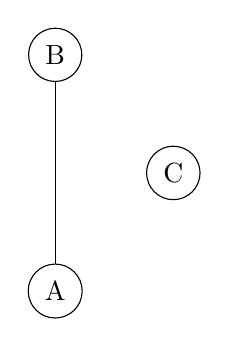
\begin{tikzpicture}
        \node[shape=circle,draw=black] (A) at (0,0) {A};
        \node[shape=circle,draw=black] (B) at (0,3) {B};
        \node[shape=circle,draw=black] (C) at (1.5,1.5) {C};

        \path [-] (A) edge node {} (B);
      \end{tikzpicture}
    \end{minipage}
  }
  \begin{itemize}
  \item Nodes are program objects
  \item (No) Edges represent (no) sharing
\end{itemize}
\end{center}
\end{frame}

\begin{frame}[fragile, c]
  \frametitle{\qub{}: Typing Environment}
  \begin{center}
    Sharing relation $\Psi$

    \begin{table}[h]
      \centering
      \begin{tabular}[c]{c c c}
      reflexive
      & $\forall x.\ x \mathbin{\Psi} x$
      & \raisebox{-0.4\height}{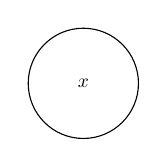
\begin{tikzpicture}[scale=0.7, fill=white, transform shape]
          \draw (0,0) circle  (1cm) node {$x$};
        \end{tikzpicture}}\\
      symmetric
      & $ \forall x, y.\ x \mathbin{\Psi} y \Rightarrow y \mathbin{\Psi} x$
      & \raisebox{-0.4\height}{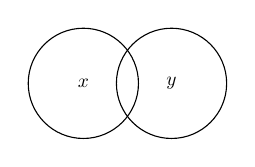
\begin{tikzpicture}[scale=0.7, fill=white, transform shape]
          \draw (0,0) circle  (1cm) node {$x$};
          \draw (1.6,0) circle  (1cm) node {$y$};
        \end{tikzpicture}}\\
      non-transitive
      & $\forall x, y, z.\ x \mathbin{\Psi} y \wedge y \mathbin{\Psi} z \not\Rightarrow x \mathbin{\Psi} z$
      & \raisebox{-0.4\height}{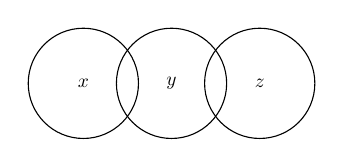
\begin{tikzpicture}[scale=0.7, fill=white, transform shape]
          \draw (0,0) circle  (1cm) node {$x$};
          \draw (1.6,0) circle  (1cm) node {$y$};
          \draw (3.2,0) circle  (1cm) node {$z$};
        \end{tikzpicture}}
      \end{tabular}
    \end{table}
\end{center}
\end{frame}

\begin{frame}[fragile, c]
  \frametitle{\qub{}: Typing Environment}
    \begin{itemize}
    \item \BI{} bunches need explicit transformations
      \begin{center}
      $ A; (B, C) \equiv (A;B),(A;C) $
      \end{center}
      \begin{center}
    {\small
      \begin{minipage}[c]{0.35\linewidth}
      \centering
      \tikzset{every tree node/.style={minimum width=2em},
        blank/.style={draw=none},
        edge from parent/.style=
        {draw,edge from parent path={(\tikzparentnode) -- (\tikzchildnode)}},
        level distance=1.5cm}
      \begin{tikzpicture}
        \Tree
        [.;
        [.,
        [.B ]
        [.C ]
        ]
        [.A ]
        ]
      \end{tikzpicture}
    \end{minipage}%
    \begin{minipage}[c]{0.2\linewidth}
      \begin{center}
      {\LARGE $\rightsquigarrow$}\\
      {\LARGE $\rightsquigarrow$}\\
      {\LARGE $\rightsquigarrow$}
    \end{center}
    \end{minipage}%
    \begin{minipage}[c]{0.45\linewidth}
      \centering
 \tikzset{every tree node/.style={minimum width=2em},
        blank/.style={draw=none},
        edge from parent/.style=
        {draw,edge from parent path={(\tikzparentnode) -- (\tikzchildnode)}},
        level distance=1.5cm}
      \begin{tikzpicture}
        \Tree
        [.,
        [.;
        [.A ]
        [.B ]
        ]
        [.;
        [.A ]
        [.C ]
        ]
        ]
      \end{tikzpicture}
    \end{minipage}
  }
\end{center}


\item \qub{} sharing graphs internalize the transformation
  \begin{center}
      {\small
    \begin{minipage}[c]{1\linewidth}
      \centering
      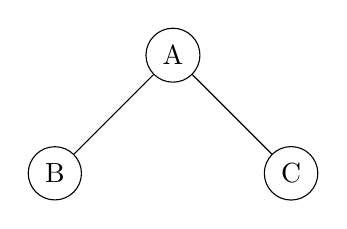
\begin{tikzpicture}
        \node[shape=circle,draw=black] (A) at (1.5,3) {A};
        \node[shape=circle,draw=black] (B) at (0,1.5) {B};
        \node[shape=circle,draw=black] (C) at (3,1.5) {C};

        \path [-] (A) edge node {} (B);
        \path [-] (A) edge node {} (C);
      \end{tikzpicture}
    \end{minipage}
  }
\end{center}

\end{itemize}
\end{frame}


\begin{frame}
  \frametitle{\qub{}: Typing Environment}
  \begin{center}
    Adjacency lists for sharing graphs

    ``$x$ of type $\sigma$ is in sharing with $\vec{y}$''

    $(x, \sigma, \vec{y}) \in \Gamma$
    \begin{flalign*}
      \text{Typing Context}\ \ \      \Gamma,\Delta     &::= \epsilon \mid \Gamma, x^{\vec{y}}:\sigma
    \end{flalign*}

  \end{center}
\end{frame}


%%% Local Variables:
%%% mode: latex
%%% TeX-master: "defense-slides"
%%% End:
